\documentclass[]{usiinfbachelorproject}


%Packages
\captionsetup{labelfont={bf}}



%opening
\title{Spectrally Accurate Resampling of High Quality Rotated Images}
\author{Dylan Reid Ramelli}



\versiondate{\today}

\begin{committee}
	\advisor[Universit\`a della Svizzera Italiana, Switzerland]{Prof}{Rolf}{Krause}
	\assistant[Universit\`a della Svizzera Italiana, Switzerland]{Dr}{Patrick}{Zulian}
	\assistant[Universit\`a della Svizzera Italiana, Switzerland]{Dr}{Diego}{Rossinelli}
\end{committee}

\abstract {
	
}

\begin{document}
	
	\maketitle	
	\section{Introduction, Motivation}\label{introduction}
	For many years the amount of digital imaging data has been increasing exponentially (citation) and as such the need for acquiring this large data and process it with care has become a central point of focus. The goal of this project is to process high quality signals, in this case images, by rotating them using techniques such as the Fourier Transform, Shift Theorem, FIR filtering and CUDA parallel processing.
		
		
	WHY, WHAt for? See applications:
	
	The accurate rotation of images is very useful in applications such as Data Augmentation for Convoluted Neural Networks, where one might have to rotate an image multiple times at random before feeding it to the neural network.  Or even in Data Visualization for multi-modal imaging. In this case we can either acquire images at different times and then combine them together so that we can manipulate the images by rotation for example to align them correctly.
	
	1D Translations cornerstone of 2D Translations which are the cornerstone for 3D translations.
	
	FT: Direct solver instead of iterative, takes in a lot of data.
	
	Applications:
	\begin{itemize}
		\item Data augmentation, for training in CNN
		\item Data visualization, multi-model imaging.
	\end{itemize}
	
	\section{State of the art}
	For certain applications such as... it is required to be able to rotate images while maintaining the highest quality possible. To achieve satisfying results the general approach is to use bilinear and nearest neighbour interpolation.
	
	
	Include images from Diego of blood vessels in the heart iI think
	
	
	\iffalse
	
	\subsection{Interpolation}
	Sampled version of our translated signal is:
	\begin{equation}
		(T_\Delta s)[k] = \sum_{l \in Z}^{} c(l)\varphi(k - \Delta - l)
	\end{equation}
	Where $\varphi$ is our generating function.
	\subsubsection{Linear Interpolation}
	With linear interpolation we want to estimate the coordinates of a point from a given number of samples. 
	
	Linear interpolation model of function sin(x) with $N = 2$:
	\begin{equation}
		\beta^1(x) = 
		\begin{cases}
			1 - |x|, & |x| < 1    \\
			0,       & otherwise, 
		\end{cases}
	\end{equation}
	\begin{center}
		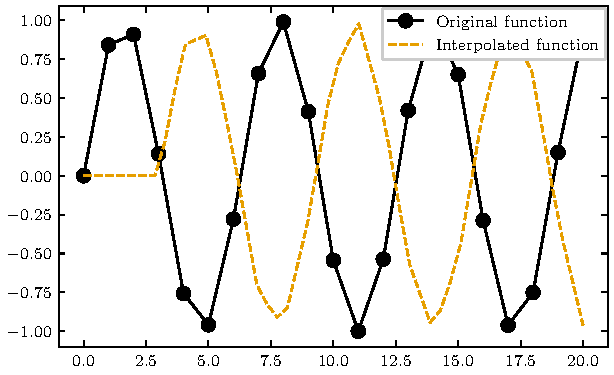
\includegraphics{"images/linear_interpolation_example.pdf"}
	\end{center}
	
	Cubic spline interpolation model of function sin(x) with $N=4$:
	\begin{equation}
		\beta^3(x) = 
		\begin{cases}
			2/3 - |x|^2 + |x|^3/2, & 0 \leq|x| < 1  \\
			(2-|x|)^3/6,           & 1 \leq |x| < 2 \\
			0,                     & 2 \leq |x|     
		\end{cases}
	\end{equation} \cite{main_article}
	
	\begin{center}
		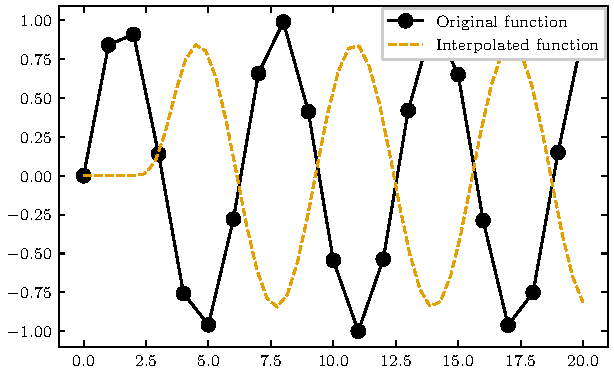
\includegraphics{"images/cubic_interpolation_example.pdf"}
	\end{center}
	
	Standard 2-D interpolation formula for computing the value of the image at location $(x,y)$
	\begin{equation}
		s(x,y) = \sum_{k = k_0}^{k_0+L-1}\sum_{l=l_0}^{l_0+L-1} c(k,l)\varphi(x-k)\varphi(y-l)
	\end{equation}
	
	\fi
	

	\section{Project Requirements}
	To complete this project I made use of different tools such as, Python, Jupyter Notebook, C/C++ and CUDA.
	
	
	
	\subsection{Frequencies of a signal}
	\begin{equation}
		freq_{n} = \lfloor \frac{n}{2} \rfloor + 1
	\end{equation}
	Visual representation with $n=3$ of the discrete Fourier transform of a function $g(x)$
	
	\begin{equation*}
		G_m = \displaystyle\sum_{k=0}^{N-1}g(k)e^{-i \frac{2\pi}{N}km}
	\end{equation*}
	
	To shift a signal by a fractional amount it is imperative to use the correct frequency when doing so.
	
	Given that for $n$ samples we have $\lfloor \frac{n}{2} \rfloor + 1$ distinct frequencies
	
	
	\begin{figure}
		\centering
		\include{file}
		\caption{Unit circle with N = 3, }
	\end{figure}
	
	Euler's Formula
	\begin{equation}
		e^{ix} = cos(x)  + i sin(x)
	\end{equation}
	
	
	\subsection{Fourier Transform with Shift Theorem}
	Given $K=4$ samples of a random function we can calculate the Fourier transform to find the values at each frequency.
	Any function(signal) has exactly $\lfloor \frac{N}{2}\rfloor+1$ distinct frequencies, but in the Fourier transform we use $M=N$ Frequencies.
	\paragraph{Example}
	$g_k = [1,0,-1,0]$, i.e the cos() function values when sampling the function with a period $T=2\pi$ at 4 evenly spaced intervals of $\pi/2$
	
	To find the amplitudes of each frequency m of M we can do:
	\begin{equation*}
		G_m = \displaystyle\sum_{k=0}^{N-1}g_k[k]e^{-i \frac{2\pi}{N} km}
	\end{equation*}
	
	Now instead of $g_k[k]$, we want $g_k[k - \delta]$
	so the above equation can be rewritten as:
	\begin{equation*}
		H_m = \displaystyle\sum_{k=0}^{N-1}g_k[k - \delta]e^{-i \frac{2\pi}{N} km}
	\end{equation*}
	
	\begin{equation*}
		H_m = \displaystyle\sum_{r = 0 - \delta}^{N-1-\delta}g_k[r]e^{-i \frac{2\pi}{N} km}, r = k - \delta 
	\end{equation*}
	
	Since $r = k - \delta$ then $ k = r + \delta$ and as such:
	
	\begin{equation*}
		H_m = \displaystyle\sum_{r= -\delta}^{N-1 - \delta}g_k[r]e^{-i \frac{2\pi}{N} (r + \delta)m}
	\end{equation*}
	
	We can then separate the exponential:
	
	\begin{equation*}
		H_m = \displaystyle\sum_{r= -\delta}^{N-1 - \delta}g_k[r]e^{-i \frac{2\pi}{N} rm}e^{-i \frac{2\pi}{N}  \delta m}
	\end{equation*}
	
	Ann factor it out of the sum:
	
	\begin{equation*}
		H_m = e^{-i \frac{2\pi}{N}  \delta m} \displaystyle\sum_{r= -\delta}^{N-1 - \delta}g_k[r]e^{-i \frac{2\pi}{N} rm}
	\end{equation*}
	
	The sum now is exactly the same as before but with a different range and value for f. We can now try it out in python.
	
	\begin{equation*}
		H_m = e^{-i \frac{2\pi}{N}  \delta m} \displaystyle\sum_{k=0}^{N-1}g_k[k]e^{-i \frac{2\pi}{N} km}
	\end{equation*}
	
	\begin{equation}
		H_m = e^{-i \frac{2\pi}{N}  \delta m} G_m
	\end{equation}
	
	The above equation works well for non fractional shifts but has problems when we want to shift by a fractional amount.
	"Explain why".\\
	To solve this we need to take into consideration the negative frequencies and in particular if the number of samples is odd or even.
	
	Normally for M frequencies we 

	
	\begin{figure}[h]
		\centering
		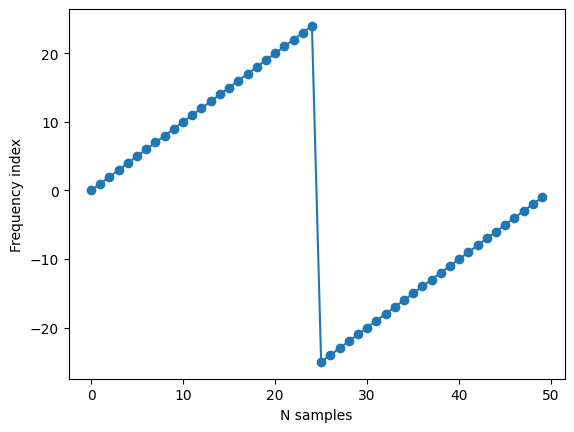
\includegraphics[width=0.7\columnwidth]{images/wavenum_n50.png}
		\caption{Wave numbers for N = 50}
	\end{figure}
	
	
	\subsection{Lanczos Filter and FIR}
	To alleviate the problems that arise when shifting a signal by a fractional amount we can use a filter that is convoluted with the shifted signal.
	
	
	
	
	\section{Project Design}
	Explain 1D,2D,3D transposition.
	Simplification of 2D rotation using 1D translations.
	
	
	
	\section{Implementation}
	\begin{itemize}
		\item Problems while implementing the code
		\item Indexing frequencies...
		\item practical problems...
	\end{itemize}
	
	\section{Result}
	
	
	\begin{itemize}
		\item Rotate image many times like in the paper
		\item look for artefacts
		\item compare with C code gathernoloss.c
		\item quality, quantity
	\end{itemize}
	
	
	\section{Solution}
	\section{Validation}
	\section{Conclusion}
	\begin{itemize}
		\item Summary
		\item limitations
	\end{itemize}
	\bibliographystyle{plain}
	\bibliography{references}
	
\end{document}